\section{Solving unseen geometric problems via hypothesis tree search}
\label{sec:unseen_levels}
In the previous section, we have shown how to train a visual recognition model to predict the next step of a given construction from a large number of examples of the same construction with different geometric configurations of the primitives. In this section, we investigate how to solve new problems, which we have not seen at training time.
This is achieved by (i) using models trained for different construction problems (see Section~\ref{mrcnn_section}) to generate {\em a set of hypotheses} for each construction step of the new problem and then (ii) searching the tree of possible constructions. These two parts are described next. 

\subsection{Generating action hypotheses}
Each primary detection from the \maskrcnn model (see Section \ref{position_dependent_pars}) can be transformed into an action.
We denote each action, its arguments, and results as a \emph{hypothesis}.
The result of an action contains a geometric primitive, constructed during the action execution, and a reward, indicating whether the output primitive is a part of the remaining goal or not.
If an action constructs a part of the goal, the reward is $1/n$, where $n$ is the total number of primitives in the initial goal, otherwise it is equal to zero.
Fig.~\ref{fig:hypotheses_explorer_hypothesis3} shows a hypothesis that successfully constructs one of the four lines in the goal and its reward thus equals $0.25$.


We can extract multiple actions from the \maskrcnn model output by considering multiple output candidate detections, transform them into multiple hypotheses, and explore their construction space.
We can also utilize hypotheses from models trained for different tasks. However, the \maskrcnn scores are not comparable across hypotheses from different models, so in a setup with multiple models we have to search even hypotheses with lower scores.
\subsection{Tree search for exploring construction hypotheses}
\label{hypotheses_tree_search}
We use tree search to explore the hypothesis space given by the predictions from one or more \maskrcnn models.
The tree search has to render the input image and obtain predictions from all considered \maskrcnn models in each node of the tree, which increases the time spent in one node.
However, as a result, we search only within the space of hypotheses output by the \maskrcnn models, which is much smaller than the space of all possible constructions.
We use iterative deepening, which is an iterated depth-limited search over increasing depth (see Algorithm~\ref{alg:IDDFS}).

\begin{figure}[!htb]
     \centering
     \begin{subfigure}[t]{0.32\textwidth}
         \centering
         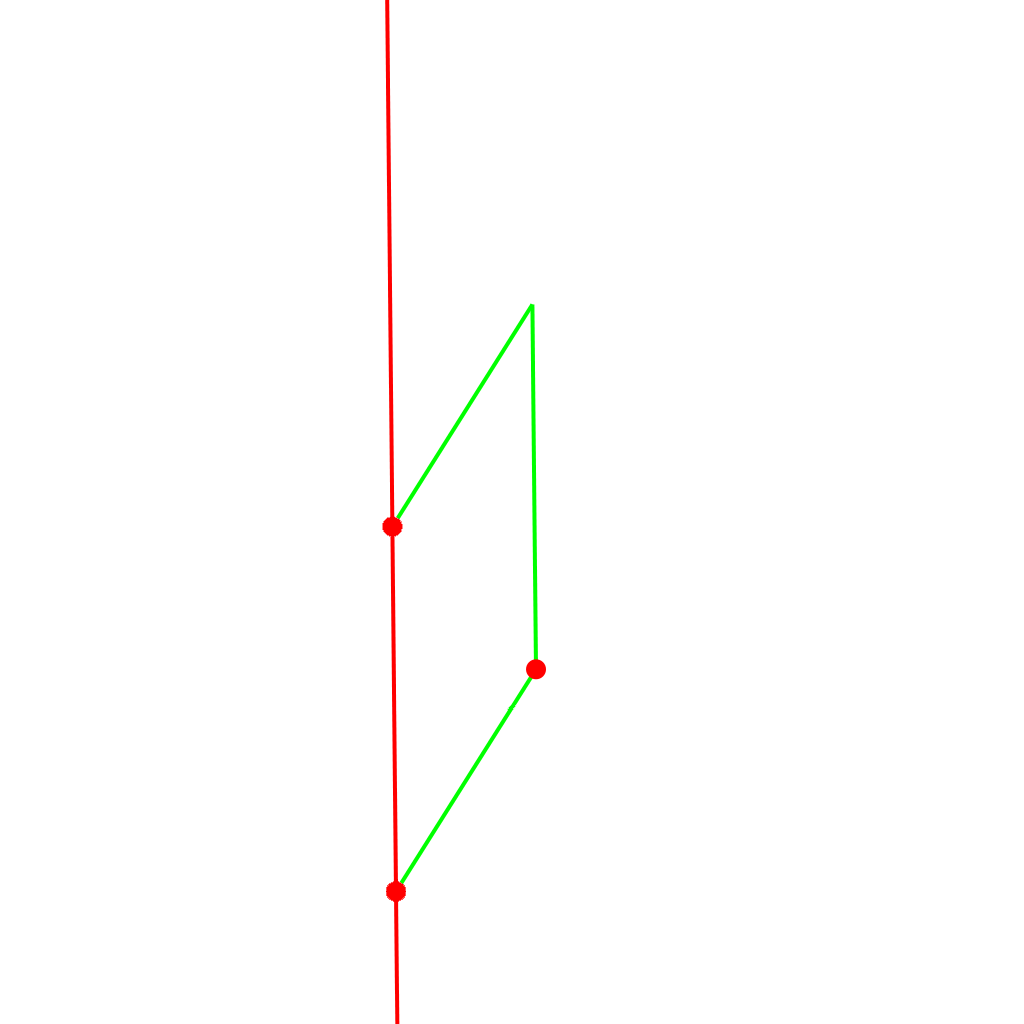
\includegraphics[width=\textwidth]{img/hypothesis_explorer/input.png}
         \caption{Current state}
         \label{fig:hypotheses_explorer_input}
     \end{subfigure}
     \hfill
     \begin{subfigure}[t]{0.32\textwidth}
         \centering
         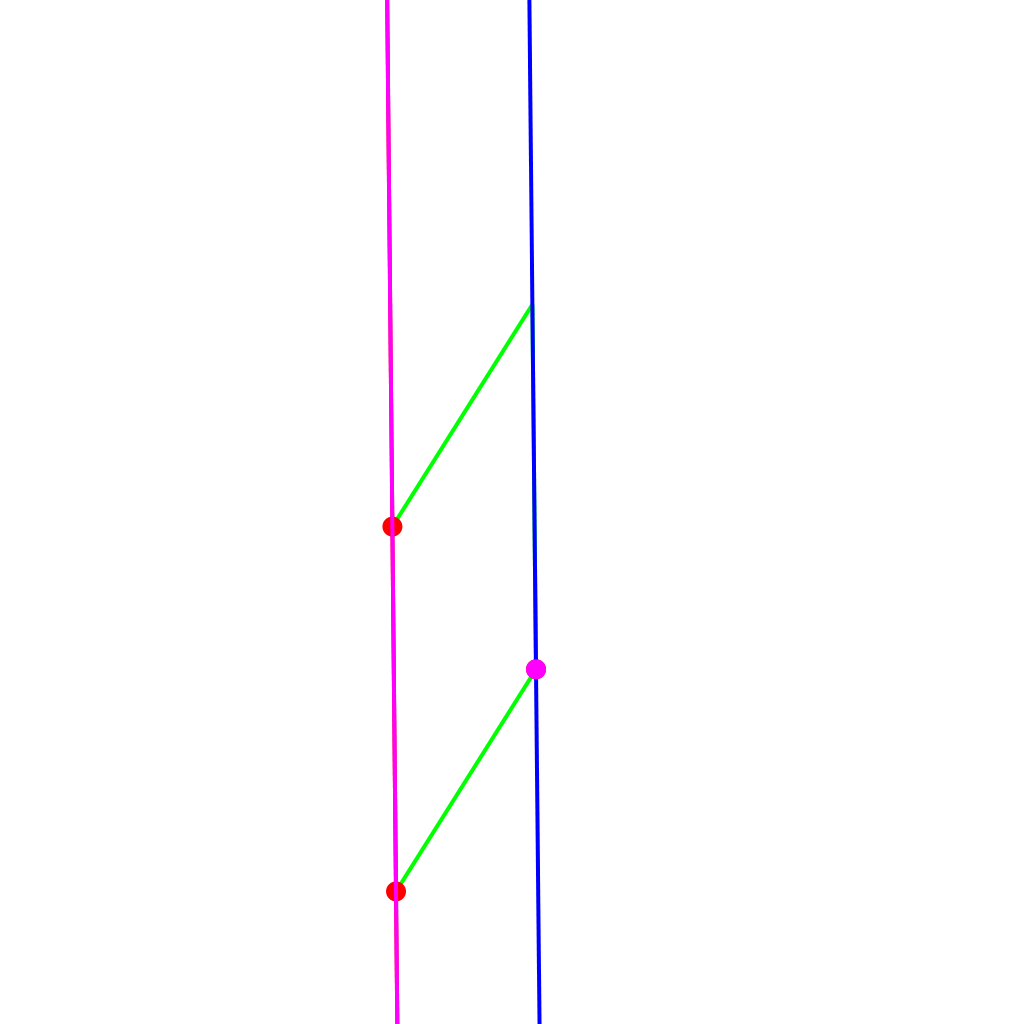
\includegraphics[width=\textwidth]{img/hypothesis_explorer/source_07_score_0_999_Parallel.png}
         \caption{Hypothesis, reward $0.65$}
         \label{fig:hypotheses_explorer_hypothesis3}
     \end{subfigure}
     \hfill
     \begin{subfigure}[t]{0.32\textwidth}
         \centering
         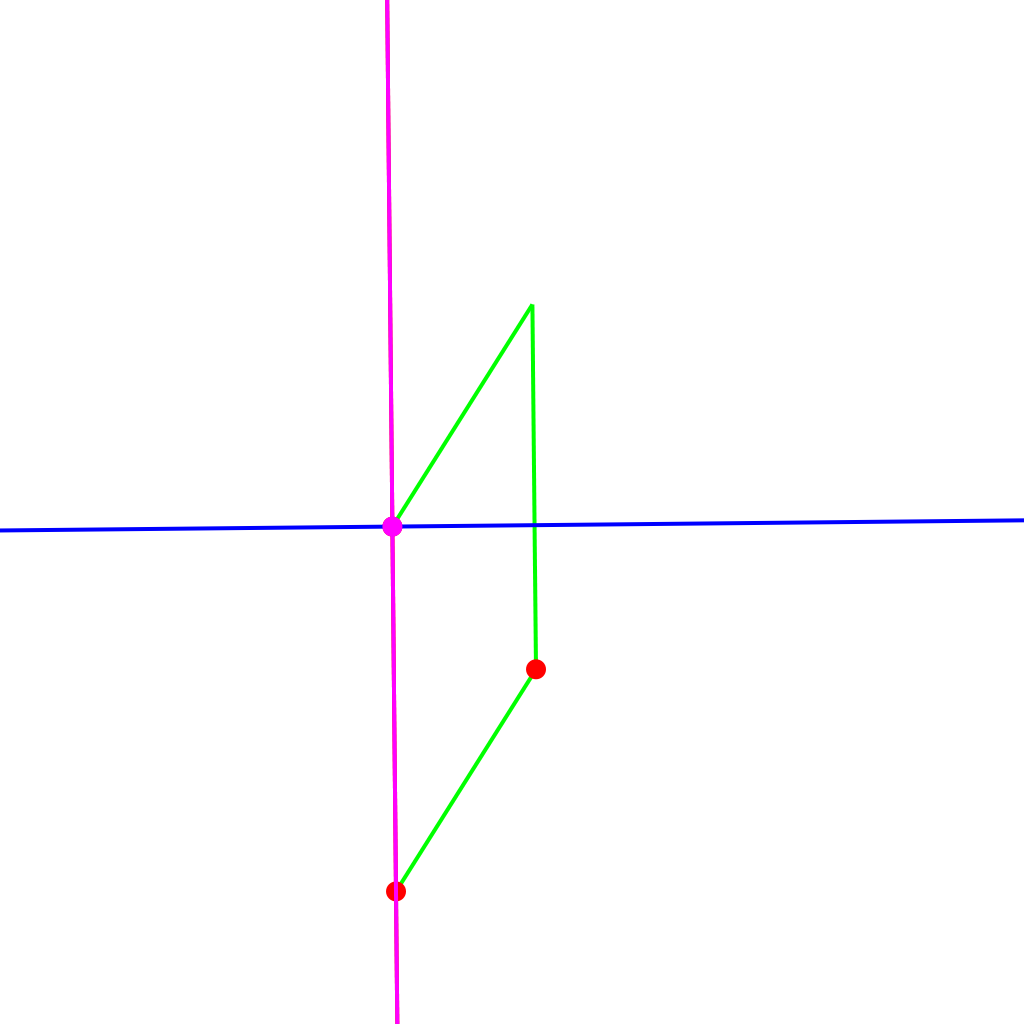
\includegraphics[width=\textwidth]{img/hypothesis_explorer/source_01_score_0_999_Perp.png}
         \caption{Hypothesis, reward $0$}
         \label{fig:hypotheses_explorer_hypothesis1}
     \end{subfigure}
     \hfill
     \begin{subfigure}[t]{0.32\textwidth}
         \centering
         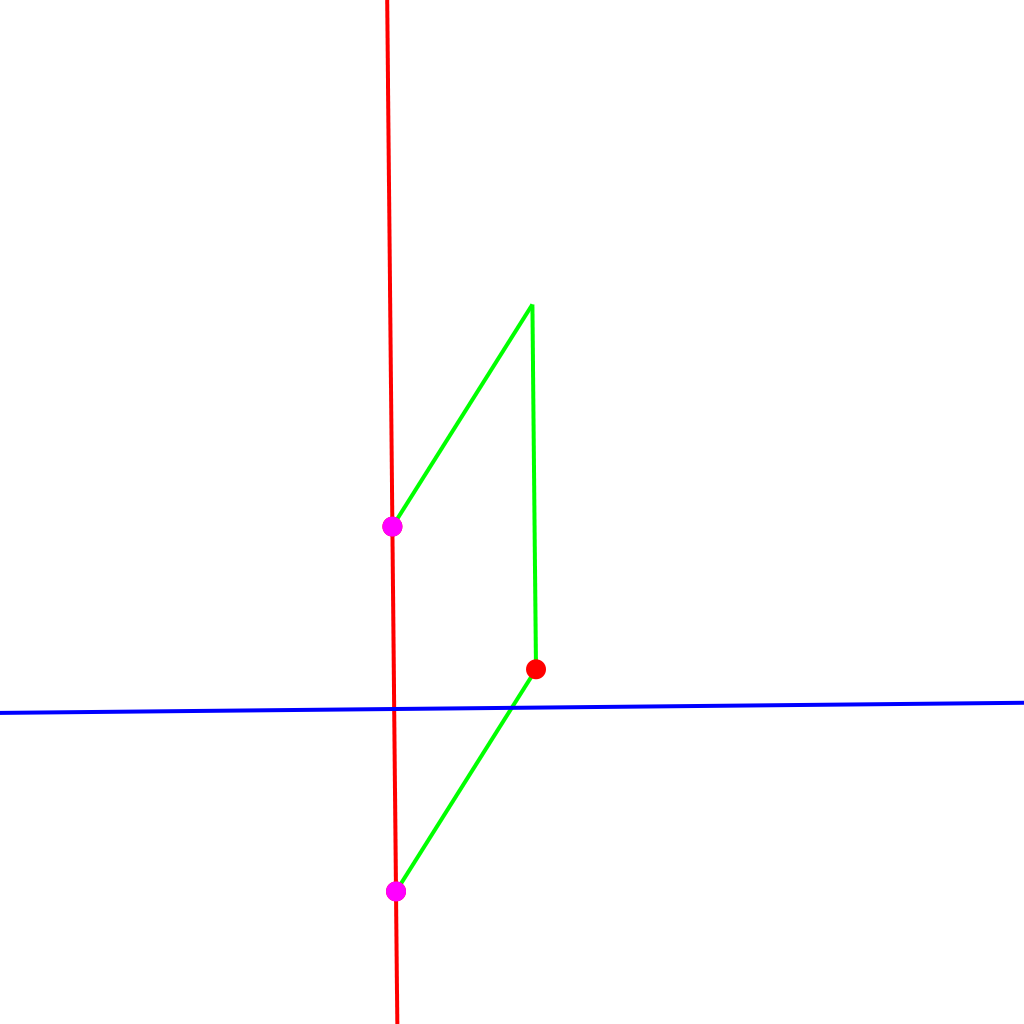
\includegraphics[width=\textwidth]{img/hypothesis_explorer/source_05_score_0_996_PerpBisector.png}
         \caption{Hypothesis, reward $0$}
         \label{fig:hypotheses_explorer_hypothesis2}
     \end{subfigure}
     \hfill
     \begin{subfigure}[t]{0.32\textwidth}
         \centering
         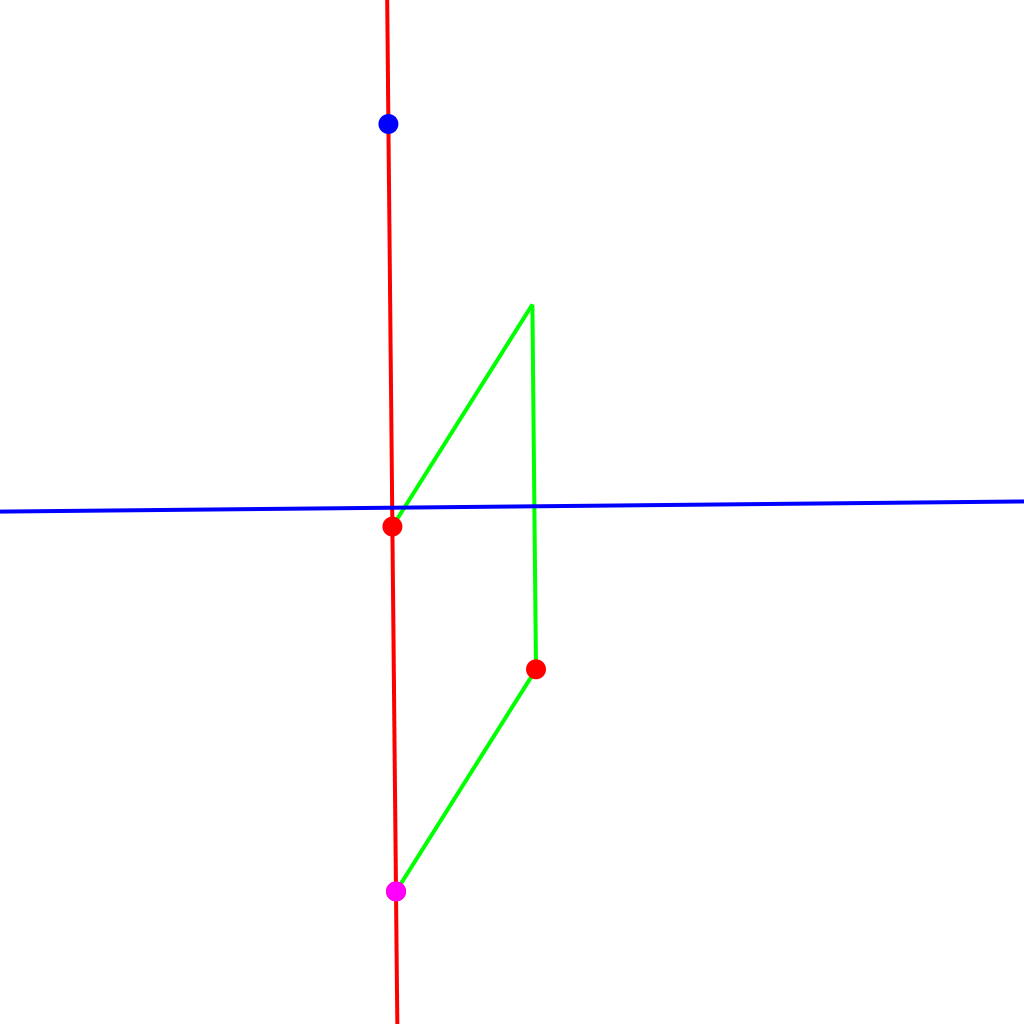
\includegraphics[width=\textwidth]{img/hypothesis_explorer/source_08_score_0_77_PerpBisector.png}
         \caption{Hypothesis, reward $0$}
         \label{fig:hypotheses_explorer_hypothesis4}
     \end{subfigure}
     \hfill
     \begin{subfigure}[t]{0.32\textwidth}
         \centering
         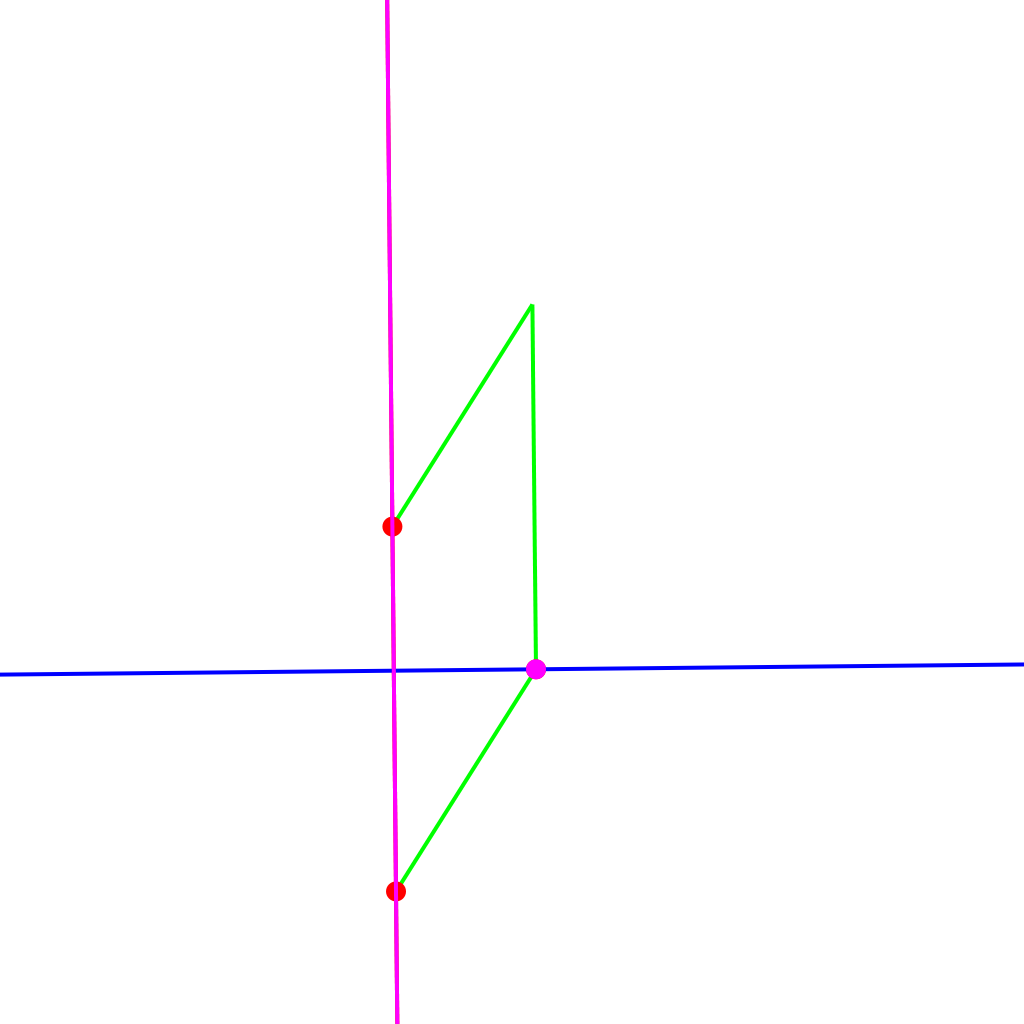
\includegraphics[width=\textwidth]{img/hypothesis_explorer/source_01_score_0_999_Perpl.png}
         \caption{Hypothesis, reward $0$}
         \label{fig:hypotheses_explorer_hypothesis5}
     \end{subfigure}
        \caption{Multiple hypotheses for the next step in Euclidea level \textit{Epsilon-03} (construct a parallelogram whose three of four vertices are given). (a) Current state. (b) Hypothesis with reward $0.25$ that constructs one of the four lines in the goal (green). (c-f) Hypotheses with reward $0$. Each image contains the current state (red), remaining goal (green), hypothesis produced by \maskrcnn (blue), and
        parameters of the tool (purple). For example, hypothesis (b) selects the Parallel tool to construct the blue line as parallel to the purple line and intersecting the purple point. A positive reward indicates contribution to the goal, so we select the hypothesis (b), which has the highest reward.
        }
        \label{fig:hypotheses_explorer}
\end{figure}

\begin{small}
\begin{algorithm}[!htb]
\SetAlgoLined
\DontPrintSemicolon
\SetAlFnt{\small\sf} 
\KwResult{Solve level with Iterative Deepening.}

    \SetKwFunction{FMain}{IterativeDeepening-DFS}
    \SetKwProg{Fn}{Function}{:}{}
    \Fn{\FMain{$InitialState$}}{
        SolutionMaxLength $\longleftarrow 0$;
        
        Solution $\longleftarrow$ \textbf{null};
        
        \While{
        (Solution = \textbf{null}) and (SolutionMaxLength $<$ MaxIterationDepth)
        }
        {
        $SolutionMaxLength \longleftarrow SolutionMaxLength +1$;
        
        Solution $\longleftarrow$ FindSolution($InitialConfig$, SolutionMaxLength);
        
        }
        \textbf{return} Solution
}
\SetKwFunction{FMain}{FindSolution}
    \SetKwProg{Fn}{Function}{:}{}
    \Fn{\FMain{$CurrentState, Depth$}}{
        \If {CurrentState.IsTheGoal}
        {\textbf{return} success \tcp{collect solution on the backtracking}}
        \If{Depth $= 0$ }{\textbf{return null} \tcp{e.g.,~solution not found.}}
        
        $Hypotheses \longleftarrow Models.GetAllHypotheses(CurrentState)$;
        
        \tcp{Hypotheses sorted in the order: Reward, Confidence score}
        
        \ForEach{$h \in Hypotheses$}
            {
            $NewState \longleftarrow Apply(h, CurrentState)$;
            
            $Solution = FindSolution(NewState, Depth -1)$;
            
            \If {Solution $\neq$ \textbf{null}}
                {\textbf{return} Solution}
            }
        \textbf{return null}
        
        

}
\vspace{2mm}
\caption{\small{Tree search for exploring construction hypotheses using Iterative Deepening Depth-First Search algorithm.}}
\label{alg:IDDFS}
\end{algorithm}
\end{small}
\label{reducing_hypotheses}
Hypotheses produced by different \maskrcnn models increase the branching factor and thus also the search time.
To speed up the tree search, we group all mutually similar hypotheses and explore only one of them.
For this purpose, we consider two hypotheses as similar if their output geometric primitive is the same; note that such hypotheses can have different arguments, including different tools.
